\documentclass{article}

\usepackage[utf8]{inputenc}
\usepackage[T1]{fontenc}
\usepackage[portuguese]{babel}
\usepackage{amsmath, amsthm, amssymb}
\usepackage{graphicx}
\usepackage{bbm}

\author{Esdras R. Carmo - 170656}
\title{Aula PED de Integrais Duplas sobre Coord. Polares}
\date{\today}

% Comando para integral dupla sobre região R
\newcommand{\doubleint}[1] {\iint\limits_R #1 dA}
\newcommand{\doubleintp}[1] {\iint\limits_{R_{r\theta}} #1 r dr d\theta}

\begin{document}
    \maketitle

    \section{Exerc. 09 Lista 7}
        \paragraph{}
        Calcule a área fora do círculo $r = 3\cos{\theta}$ e dentro de $r = 1 + \cos{\theta}$.

        Precisamos calcular
        \[
            \doubleint{} = \doubleintp{}
        \]

        Plotando os dois gráficos em coordenadas polares, temos:

        \begin{figure}[h!]
            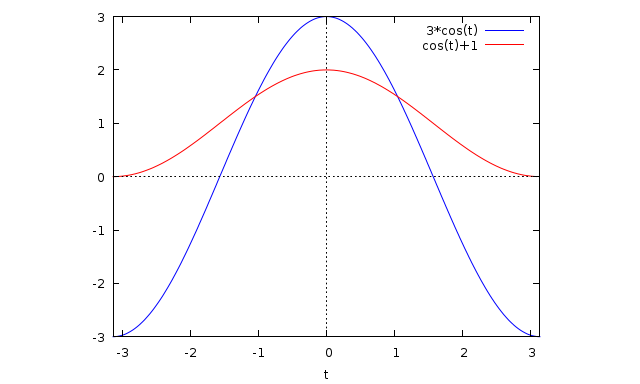
\includegraphics[width=\linewidth]{cos.png}
        \end{figure}

        Desconsiderando a parte em que $r < 0$, pois não possui significado geométrico,
        temos duas regiões simétricas e podemos calcular a integral de apenas uma e multiplicar
        por 2.

        Dessa forma, podemos encontrar as duas regiões que formam a parte positiva:

        \begin{align*}
            1 + \cos{\theta} &= 3\cos{\theta}\\
            \cos{\theta} &= \frac{1}{2}\\
            \theta &= \frac{\pi}{3} \textit{, pois } -\pi \leq \theta \leq \pi
        \end{align*}

        Assim temos as regiões:

        \begin{align*}
            R_1 &:= \{(r, \theta) \mid \frac{\pi}{3} \leq \theta \leq \frac{\pi}{2}, 3\cos{\theta} \leq r \leq 1 + \cos{\theta} \}\\
            R_2 &:= \{(r, \theta) \mid \frac{\pi}{2} \leq \theta \leq \pi, 0 \leq r \leq 1 + \cos{\theta} \}
        \end{align*}

        E podemos integrar:

        \begin{align*}
            V &= 2 \doubleintp{}\\
            V &= 2 \left( \int_{\frac{\pi}{3}}^{\frac{\pi}{2}} \int_{3 \cos{\theta}}^{1 + \cos{\theta}} r dr d\theta + \int_{\frac{\pi}{2}}^{\pi} \int_{0}^{1 + \cos{\theta}} r dr d\theta \right)\\
            V &= \frac{\pi}{4}
        \end{align*}

    \section{Exerc. 10 Lista 7}
        \paragraph{}
        Calcule o volume do sólido limitado pelo cone $z^2 = x^2 + y^2$ e pelo cilindro $x^2 + y^2 = x$.

        Encontramos o centro da circunferência que determina o cilindro:

        \begin{align*}
            x^2 - x + y^2 &= 0\\
            x^2 - x + \frac{1}{4} + y^2 &= \frac{1}{4}\\
            \left( x - \frac{1}{2} \right)^2 + y^2 &= \frac{1}{4}\\
        \end{align*}

        Note que o cone possui apenas o ponto $(0, 0, 0)$ no plano $xy$. Além disso,
        ele é simétrico em relação ao plano $xy$, logo podemos definir a região de
        integração como a circunferência geradora do cilindro e o volume será a integral
        da parte positiva multiplicada por 2.

        Então, transformando em coordenadas polares temos:

        \begin{align*}
            x^2 + y^2 &= x \Rightarrow r = \cos{\theta}\\
        \end{align*}

        Vamos integrar $z = +\sqrt{ x^2 + y^2 }$:

        \begin{align*}
            V &= 2 \doubleintp{r}\\
            V &= 2 \int_{\frac{-\pi}{2}}^{\frac{\pi}{2}} \int_0^{\cos{\theta}} r^2 dr d\theta\\
            V &= \frac{2}{3} \int_{\frac{-\pi}{2}}^{\frac{\pi}{2}} \cos^3{\theta} d\theta\\
            V &= \frac{2}{3} \left\{ \left[ \sin{\theta} \right]_{-\frac{\pi}{2}}^{\frac{\pi}{2}} - \left[ \frac{\sin^3{\theta}}{3} \right]_{-\frac{\pi}{2}}^{\frac{\pi}{2}}  \right\}
        \end{align*}
\end{document}
